\documentclass{beamer}
\usetheme{Warsaw}

\usepackage{graphicx} % Allows including images
\usepackage{booktabs} % Allows the use of \toprule, \midrule and \bottomrule in tables
\usepackage{listings}
\usepackage[utf8]{inputenc}
\usepackage[overlay,absolute]{textpos}

\AtBeginSection[]
{
\begin{frame}<beamer>
\frametitle{Plan}
\tableofcontents[
  currentsection,
  sectionstyle=show/show,
  subsectionstyle=hide
]
\end{frame}
}

\lstset{language=C++,
                basicstyle=\ttfamily,
                keywordstyle=\color{teal}\ttfamily,
                stringstyle=\color{red}\ttfamily,
                commentstyle=\color{cyan}\ttfamily,
                morecomment=[l][\color{magenta}]{\#}
}

\setbeamercolor{normal text}{fg=white,bg=black!90}
\setbeamercolor{structure}{fg=white}

\setbeamercolor{alerted text}{fg=red!85!black}

\setbeamercolor{item projected}{use=item,fg=black,bg=item.fg!35}

\setbeamercolor*{palette primary}{use=structure,fg=structure.fg}
\setbeamercolor*{palette secondary}{use=structure,fg=structure.fg!95!black}
\setbeamercolor*{palette tertiary}{use=structure,fg=structure.fg!90!black}
\setbeamercolor*{palette quaternary}{use=structure,fg=structure.fg!95!black,bg=black!80}

\setbeamercolor*{framesubtitle}{fg=white}

\setbeamercolor*{block title}{parent=structure,bg=black!60}
\setbeamercolor*{block body}{fg=black,bg=black!10}
\setbeamercolor*{block title alerted}{parent=alerted text,bg=black!15}
\setbeamercolor*{block title example}{parent=example text,bg=black!15}

\author[Félix-Antoine Ouellet]{Félix-Antoine Ouellet}

\title[PGAS\hspace{2em}\insertframenumber/\inserttotalframenumber]{Espace d'addressage global partitionné}

\institute{Université de Sherbrooke}

\date{2 octobre 2014}

\begin{document}

\begin{frame}
\titlepage % Print the title page as the first slide
\end{frame}

\section{Motivation}
\subsection{État présent du matériel}
\begin{frame}
\frametitle{Explosion de parallélisme}
\framesubtitle{Superordinateurs}
\begin{itemize}
\item Aux portes de l'\textit{exascale computing}
\item $10^{18}$ opérations en virgule flottante par seconde
\item Potentiellement 1 milliard de \textit{threads} à gérer simultanément
\end{itemize}
\end{frame}

\begin{frame}
\frametitle{Explosion de parallélisme}
\framesubtitle{Appareils courants}
\begin{itemize}
\item Processeurs vectoriels
\item Processeurs multi-coeurs
\item Accélérateurs
\end{itemize}
\end{frame}

\subsection{État présent du logiciel}
\begin{frame}
\frametitle{Programmation parallèle avec mémoire partagée}
\begin{center}
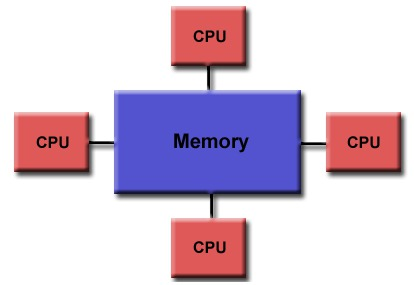
\includegraphics[scale=0.6]{sharedmem.jpg}
\end{center}
\end{frame}

\begin{frame}
\frametitle{Programmation parallèle avec mémoire partagée}
\begin{minipage}[t]{0.5\linewidth}
    \textbf{Avantages}:
    \begin{itemize}
    \item{aaa}
    \end{itemize}
    \end{minipage}%
    \begin{minipage}[t]{0.5\linewidth}
    \textbf{Inconvénients}:
    \begin{itemize}
    \item{Conditions de course}
    \end{itemize}
\end{minipage}
\end{frame}

\begin{frame}
\frametitle{Programmation parallèle avec mémoire distribuée}
\begin{center}
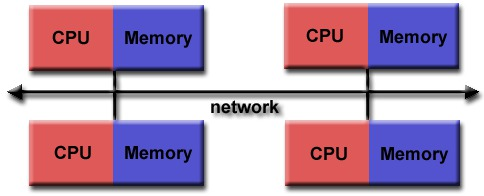
\includegraphics[scale=0.6]{distributedmem.jpg}
\end{center}
\end{frame}

\begin{frame}
\frametitle{Programmation parallèle avec mémoire distribué}
\begin{minipage}[t]{0.5\linewidth}
    \textbf{Avantages}:
    \begin{itemize}
    \item{Pas de conditions de course}
    \end{itemize}
    \end{minipage}%
    \begin{minipage}[t]{0.5\linewidth}
    \textbf{Inconvénients}:
    \begin{itemize}
    \item{Doit penser à la distribution des données}
    \end{itemize}
\end{minipage}
\end{frame}

\section{Espace d'addressage global partitionné}
\begin{frame}
\frametitle{}
\end{frame}

\section{Espace d'addressage global partitionné asynchrone}
\begin{frame}
\frametitle{}
\end{frame}

\section{Implémentation}
\begin{frame}
\frametitle{DARPA HPCS}
\begin{itemize}
\item \textit{High Productivity Computing Systems}
\item But: Produire des systèmes informatiques hautement productif pour l'industrie et la sécurité nationale
\end{itemize}
\end{frame}

\begin{frame}
\frametitle{Chapel}
\framesubtitle{Présentation}
\begin{itemize}
\item Réponse de Cray au projet HPCS
\item Inspiré de langage comme C, C++, C\#, Java, Fortran, HPF
\end{itemize}
\end{frame}

\begin{frame}
\frametitle{Chapel}
\framesubtitle{Localité}
\end{frame}

\begin{frame}
\frametitle{Chapel}
\framesubtitle{Exemple}
\end{frame}

\begin{frame}
\frametitle{HPX}
\end{frame}

\begin{frame}
\frametitle{HPX}
\framesubtitle{Exemple}
\end{frame}

\section{Conclusion}
\begin{frame}
\frametitle{Conclusion}
\end{frame}

\end{document}